\chapter{Symmetry Groups}
This chapter is central to the relevance and analysis of group theory. The core result of this chapter, Cayley's theorem, links our ideas of symmetry with the idea of groups, and how groups are a form of \textit{generalized symmetry}. It answers why group theory is oft called ``the study of symmetry'', and highlights the importance of bijections in the study of groups.

\section{Permutations}
A bijective function is too abstract an object. Such functions can take many forms. Thus, it is worth asking: what properties must a bijective function satisfy?

A bijective function is a function that maps all elements from one set to another set exactly. There are no leftovers (surjective), and each output has exactly one input that produces it (injective). In a sense, a bijective function \textit{rearranges} the elements in a set; it renames elements and shuffles them around, without destroying the relative relationships between the elements.

For bijections between finite sets, each set has the same number of elements, so it is reasonable to talk about the rearrangement and enumeration of elements in such sets.
\begin{itemize}
    \item What we mean by \textbf{rearrange} is to rename elements. We can give elements a new name and place it in the codomain.
    \item What we mean by \textbf{enumerate} is to assign each element in each finite set a unique `index number', per se. Each element can have a unique number identifying its original \textit{position} in the set, and its final position in the destination set.
\end{itemize}

Such bijections between finite sets are called \textbf{permutations}\index{permutations}, since they simply permute the `index number' of the elements in the sets.

\begin{example}
    Consider the set $S = \{1, 2, 3, 4, 5\}$. A bijection $f: S \to S$ could perform the following mapping:
    \begin{itemize}
        \item $1 \mapsto 2$;
        \item $2 \mapsto 4$;
        \item $3 \mapsto 3$;
        \item $4 \mapsto 5$; and
        \item $5 \mapsto 1$.
    \end{itemize}
    In this case, the function $f$ is said to be a permutation because the ordered list $[2, 4, 3, 5, 1]$ is one rearrangement of the items in the set $\{1, 2, 3, 4, 5\}$.
\end{example}

\begin{remark}
    It is certainly confusing that the operation of rearranging the items is also called \textit{permuting} the items in the set, and one such rearrangement is called a permutation. For groups, treat a ``permutation'' as a bijective function between finite groups.
\end{remark}

Permutations come in many different forms, but the core thing that they do is to rearrange items. From the above example, one could form a `cycle'\index{cycle} of how each item is mapped to another:
\begin{itemize}
    \item $1 \mapsto 2 \mapsto 4 \mapsto 5 \mapsto 1$; and
    \item $3 \mapsto 3$.
\end{itemize}
We can describe a permutation based on how it cycles elements. Consider this mapping performed by the map $\phi: S \to S$:
\begin{itemize}
    \item $1 \mapsto 2$;
    \item $2 \mapsto 4$;
    \item $3 \mapsto 5$;
    \item $4 \mapsto 1$; and
    \item $5 \mapsto 3$.
\end{itemize}
How $\phi$ operates on an element can be described in \textbf{cycle notation}\index{cycle!notation}. The cycle notation of a permutation may also be called its \textbf{cycle decomposition}\index{cycle!decomposition}. Here's how to describe a permutation in cycle notation.
\begin{enumerate}
    \item Start by opening a bracket: ``(''.
    \item Write the first element that has not appeared yet in the cycle notation.
    \begin{itemize}
        \item Initially, we write the number 1, so it currently is ``(1''.
    \end{itemize}
    \item Find out where that element is mapped to.
    \begin{itemize}
        \item For the case of the element 1, it is mapped to 2.
    \end{itemize}
    \item Write the mapped element next to the previous element.
    \begin{itemize}
        \item In this case, we will write ``(1 2''
    \end{itemize}
    \item Repeat steps 3 and 4 with the mapped element, until reaching an element that has already appeared in the cycle notation.
    \begin{itemize}
        \item Since 2 maps to 4, we write ``(1 2 4''
        \item Since 4 maps to 1, we terminate this process.
    \end{itemize}
    \item Close the bracket.
    \begin{itemize}
        \item So our first cycle looks like ``(1 2 4)''
    \end{itemize}
    \item Repeat steps 1 to 6 until all elements are used.
    \begin{itemize}
        \item So our final cycle notation for $g$ is ``(1 2 4)(3 5)''
    \end{itemize}
\end{enumerate}

We note some important things about this process.
\begin{itemize}
    \item Omit any elements that maps to itself. For example, if $1 \mapsto 3$, $2 \mapsto 6$, $3 \mapsto 4$, $4 \mapsto 1$, $5 \mapsto 5$, $6 \mapsto 2$, and $7 \mapsto 7$, then we ignore the 5 and 7; the corresponding cycle notation is ``(1 3 4)(2 6)''.
    \item If the permutation is the identity permutation, then it is denoted by $\id$.
\end{itemize}

\begin{example}
    Let the permutation $\alpha$ have cycle decomposition $\begin{pmatrix}1 & 3 & 5 & 2\end{pmatrix}$. Then
    \begin{multicols}{3}
        \begin{itemize}
            \item $\alpha(1) = 3$;
            \item $\alpha(2) = 1$;
            \item $\alpha(3) = 5$;
            \item $\alpha(4) = 4$;
            \item $\alpha(5) = 2$; and
            \item $\alpha(n) = n$ for $n \geq 6$.
        \end{itemize}
    \end{multicols}
\end{example}

\begin{example}
    Let the permutation $\beta$ have cycle notation $\begin{pmatrix}1 & 6 & 2 & 9 & 7 & 4\end{pmatrix}$. Then
    \begin{multicols}{3}
        \begin{itemize}
            \item $\beta(1) = 6$;
            \item $\beta(2) = 9$;
            \item $\beta(3) = 3$;
            \item $\beta(4) = 1$;
            \item $\beta(5) = 5$;
            \item $\beta(6) = 2$;
            \item $\beta(7) = 4$;
            \item $\beta(8) = 8$;
            \item $\beta(9) = 7$; and
            \item $\beta(n) = n$ for $n \geq 10$.
        \end{itemize}
    \end{multicols}
\end{example}

\begin{exercise}
    Find the cycle decomposition of the following permutations.
    \begin{partquestions}{\alph*}
        \item $1 \mapsto 2$, $2 \mapsto 3$, $3 \mapsto 1$
        \item $1 \mapsto 3$, $2 \mapsto 2$, $3 \mapsto 1$
        \item $1 \mapsto 3$, $2 \mapsto 4$, $3 \mapsto 1$, $4 \mapsto 5$, $5 \mapsto 2$
    \end{partquestions}
\end{exercise}

We now look at composing permutations\index{permutation!composing}.
\begin{example}
    Let $f$ and $g$ be permutations. Let $f$ have cycle notation $\begin{pmatrix}1 & 3 & 5 & 2\end{pmatrix}$ and $g$ have cycle notation $\begin{pmatrix}2 & 4 & 3\end{pmatrix}$. Then $h = fg$ is a permutation with
    \begin{itemize}
        \item $h(1) = f(g(1)) = f(1) = 3$;
        \item $h(2) = f(g(2)) = f(4) = 4$;
        \item $h(3) = f(g(3)) = f(2) = 1$;
        \item $h(4) = f(g(4)) = f(3) = 5$; and
        \item $h(5) = f(g(5)) = f(5) = 2$.
    \end{itemize}

    So $h$ maps 1 to 3, 2 to 4, 3 to 1, 4 to 5, and 5 to 2, meaning $h$ has cycle notation
    \[
        \begin{pmatrix}1 & 3\end{pmatrix}\begin{pmatrix}2 & 4 & 5\end{pmatrix}.
    \]
\end{example}

\begin{example}
    We have
    \[
        \begin{pmatrix}2 & 9 & 7 & 4\end{pmatrix}\begin{pmatrix}1 & 6 & 4\end{pmatrix} = \begin{pmatrix}1 & 6 & 2 & 9 & 7 & 4\end{pmatrix}.
    \]
\end{example}

We now describe how to find the inverse of a permutation\index{permutation!inverse}. Given a cycle decomposition for the permutation $f$, simply read the cycle notation backwards, ensuring that the smallest element remains at the front.

\begin{example}
    Consider the permutation $\begin{pmatrix}1 & 8 & 4 & 2\end{pmatrix}$. Its inverse is $\begin{pmatrix}2 & 4 & 8 & 1\end{pmatrix} = \begin{pmatrix}1 & 2 & 4 & 8\end{pmatrix}$.
\end{example}

\begin{example}
    $\begin{pmatrix}1 & 7 & 5 & 3 & 9\end{pmatrix}^{-1} = \begin{pmatrix}1 & 9 & 3 & 5 & 7\end{pmatrix}$.
\end{example}

\begin{exercise}
    Find the inverse of the permutation $\pi$, which has cycle notation
    \[
        \begin{pmatrix}1 & 5 & 2\end{pmatrix}\begin{pmatrix}2 & 5 & 3 & 4\end{pmatrix}.
    \]
\end{exercise}

\section{The Symmetric Group of a Set}
With the definition of permutations out of the way, we can finally introduce a very important type of group: the \textbf{symmetric group} of a set $X$.

\begin{definition}
    Let $X$ be a set. Define the \textbf{symmetric group of $X$}\index{symmetric group} by
    \[
        \Sym{X} = \{f: X \to X \vert f \text{ is a bijection}\}.
    \]
\end{definition}
\begin{proposition}
    $(\Sym{X}, \circ)$ is a group, where $\circ$ is the function composition operator.
\end{proposition}
\begin{proof}
    We prove the 4 group axioms.
    \begin{enumerate}
        \item \textbf{Closure}: Let $f$ and $g$ be functions in $\Sym{X}$, so $f: X\to X$ and $g:X \to X$ are bijective functions. Define $h:X \to X$ where $h = f\circ g$. By \myref{exercise-composition-of-isomorphisms-is-isomorphisms} we know $h$ is bijective. Thus $\Sym{X}$ is closed under $\circ$.
        
        \item \textbf{Associativity}: Function composition is associative.
        
        \item \textbf{Identity}: Clearly the identity map, $\id$, is in $\Sym{X}$. Also $\id$ is a bijection by \myref{exercise-identity-map-is-isomorphism}. Now we show that $\id$ is indeed the identity in $\Sym{X}$. Let $x$ be an arbitrary element of $X$, and $f$ be any function in $\Sym{X}$. Then
        \[
            (\id \circ f)(x) = \id(f(x)) = f(x)
        \]
        and
        \[
            (f \circ \id)(x) = f(\id(x)) = f(x)
        \]
        so $\id$ is the identity in $\Sym{X}$.
        
        \item \textbf{Inverse}: For all functions $f$ in $\Sym{X}$, $f^{-1}$ exists since $f$ is a bijection. Furthermore, $f^{-1}$ is a bijection from $X$ to $X$, so $f^{-1}$ is in $\Sym{X}$. By definition of $f^{-1}$,
        \[
            f \circ f^{-1} = f^{-1} \circ f = \id
        \]
        so $f^{-1}$ is indeed the inverse of $f$ in $\Sym{X}$.
    \end{enumerate}
    Therefore $(\Sym{X}, \circ)$ is a group.
\end{proof}

The group $(\Sym{X}, \circ)$ is called the \textbf{symmetric group} of $X$\index{symmetric group!of a set $X$}. We usually suppress the function composition operator and call $\Sym{X}$ the symmetric group of $X$.

The most relevant type of symmetric group we encounter when working with finite groups is the \textbf{symmetric group of degree $n$}\index{symmetric group!of degree $n$} (or \textbf{symmetric group of $n$ letters}\index{symmetric group!of $n$ letters}).
\begin{definition}
    The \textbf{symmetric group of degree $n$} is denoted by $\Sn{n}$ and is given by the group $\Sym{\{1, 2, 3, \dots, n\}}$.
\end{definition}
\begin{remark}
    Elements of $\Sn{n}$ are called permutations.
\end{remark}

\begin{example}\label{example-symmetric-group-of-degree-3}
    Consider the symmetric group of degree 3, $\Sn{3}$. We show all function mappings of $\Sn{3}$.

    \begin{figure}[h]
        \centering
        \fbox{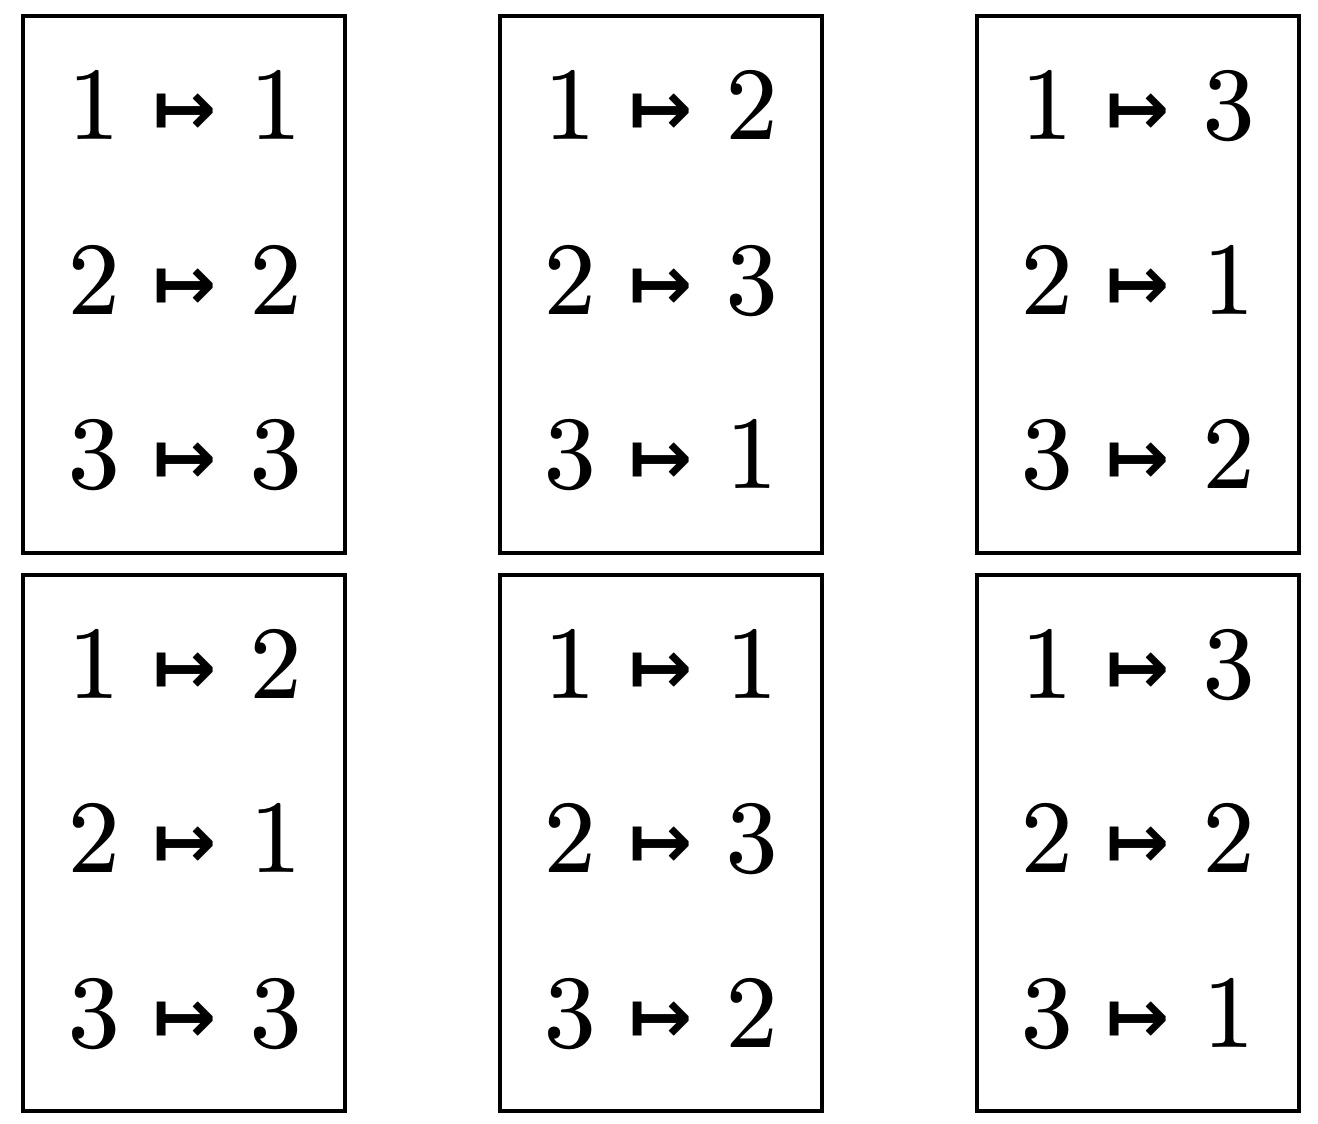
\includegraphics[width=5cm]{symmetry-groups/s3.jpg}}
        \caption{All Mappings of $\Sn{3}$}
    \end{figure}

    Thus, $|\Sn{3}| = 6$.
\end{example}
\begin{exercise}\label{exercise-order-of-Sn}
    Explain why $|\Sn{n}| = n!$.
\end{exercise}

It should also be noted that subgroups of $\Sym{X}$ are called \textbf{permutation groups}\index{permutation groups}, primarily because they contain permutations. Since a group is its own subgroup, the symmetric group may sometimes be called \textit{the} permutation group.

Finally, we prove an important result regarding symmetric groups of equal order.
\begin{theorem}\label{thrm-symmetric-groups-of-same-order-are-isomorphic}
    Let $S_1$ and $S_2$ be two finite sets with cardinality $n$. Then
    \[
        \Sym{S_1} \cong \Sym{S_2}.
    \]
\end{theorem}
\begin{proof}[Proof (see {\cite[Proof 2]{proofwiki_symmetric-group-of-same-order-are-isomorphic}})]
    Since the two sets $S_1$ and $S_2$ have the same cardinality, they have the same number of elements. Hence there exists a bijection $f: S_1 \to S_2$.

    Let $\phi: \Sym{S_1} \to \Sym{S_2}$ where $\sigma \mapsto f\sigma f^{-1}$. We show that $\phi$ is an isomorphism.
    \begin{itemize}
        \item \textbf{Homomorphism}: Let $\sigma, \pi \in \Sym{S_1}$. Then
        \begin{align*}
            \phi(\sigma\pi) &= f(\sigma\pi)f^{-1}\\
            &= f\sigma(f^{-1}f)\pi f^{-1}\\
            &= (f\sigma f^{-1})(f\pi f^{-1})\\
            &= \phi(\sigma)\phi(\pi)
        \end{align*}
        which shows that $\phi$ is a homomorphism.

        \item \textbf{Injective}: Let $\sigma, \pi \in \Sym{S_1}$ such that $\phi(\sigma) = \phi(\pi)$. Thus $f\sigma f^{-1} = f\pi f^{-1}$ which quickly implies $\sigma = \pi$ by cancellation law. Therefore $\phi$ is injective.
        
        \item \textbf{Surjective}: Let $\pi \in \Sym{S_2}$. Let $\sigma = f^{-1}\pi f$. We note that $\sigma: S_1 \to S_1$ is a bijection, so $\sigma \in \Sym{S_1}$. Clearly
        \[
            \phi(\sigma) = \phi(f^{-1}\pi f) = f(f^{-1}\pi f)f^{-1} = \pi
        \]
        so $\sigma$ is the pre-image of $\pi$. Hence $\sigma$ is the pre-image of $\pi$.
    \end{itemize}
    Therefore $\phi$ is an isomorphism, which means that $\Sym{S_1} \cong \Sym{S_2}$.
\end{proof}

\begin{corollary}\label{corollary-symmetric-group-of-finite-order}
    If the set $A$ is finite with cardinality $n$ then $\Sym{A} \cong \Sn{n}$.
\end{corollary}
\begin{proof}
    Let $X = \{1, 2, 3, \dots, n\}$. We note that $\Sn{n} = \Sym{X}$ by definition, and that $|X| = n$. We also note that $|A| = n$ so $A$ and $X$ are two finite sets with equal cardinality. Result follows from \myref{thrm-symmetric-groups-of-same-order-are-isomorphic}.
\end{proof}

\section{Cayley's Theorem}
We now have sufficient background to state and prove Cayley's theorem.

\begin{theorem}[Cayley]\label{thrm-cayley}\index{Cayley's Theorem}
    Every group is isomorphic to a permutation group.
\end{theorem}

The statement of the theorem, although simple, is the reason \textit{why} group theorists study group theory: to explore all the ways that a group can be symmetric.

The proof of this theorem is involved and technical, but we'll try and simplify its proof as much as possible.

\begin{proof}[Proof (cf. {\cite[Proof 2]{proofwiki_cayleys-theorem}})]
    Let $G$ be any group. We want to prove that there exists a group of bijective functions from $G$ to $G$ that is isomorphic to $G$ (i.e., a permutation group).

    For any $g$ in $G$ define the map $\lambda_g: G \to G$ such that $x \mapsto gx$. We claim that $\lambda_g$ is a bijection.
    \begin{itemize}
        \item \textbf{Injective}: Let $x$ and $y$ be elements of $G$ such that $\lambda_g(x) = \lambda_g(y)$. Then $gx = gy$ by definition of $\lambda_g$, which immediately means $x = y$ by cancellation law. Thus $\lambda_g(x) = \lambda_g(y)$ implies $x = y$, meaning $\lambda_g$ is injective.
        
        \item \textbf{Surjective}: Let $y$ be an element of $G$. Note that $g^{-1}y$ is an element of $G$ (since $G$ is closed), and that $\lambda_g(g^{-1}y) = g(g^{-1}y) = y$. Thus, a preimage of $y$ is $g^{-1}y$ and it exists in the domain $G$, meaning $\lambda_g$ is surjective.
    \end{itemize}
    Since $\lambda_g$ is both injective and surjective it is thus bijective.

    Now let $H = \{\lambda_g \vert g \in G\}$. Since $\lambda_g$ are all bijections from $G$ to $G$, thus $H \subseteq \Sym{G}$. We show that $H \leq \Sym{G}$ via the subgroup test.

    We first note that $\lambda_e = \id$ since
    \[
        \lambda_e(x) = ex = x = \id(x)
    \]
    for all $x$ in $G$, meaning $\id = \lambda_e \in H$. Also, the inverse of any function $\lambda_g$ is $\lambda_{g^{-1}}$ since
    \[
        (\lambda_g \circ \lambda_{g^{-1}})(x) = gg^{-1}x = x = \lambda_e(x)
    \]
    and
    \[
        (\lambda_{g^{-1}} \circ \lambda_g)(x) = g^{-1}gx = x = \lambda_e(x).
    \]
    Now suppose $\lambda_{g_1}, \lambda_{g_2} \in H$ (where $g_1, g_2 \in G$). Note $g_1g_2^{-1}$ is an element of $G$ since $G$ is closed. Therefore, for all $x$ in $G$,
    \begin{align*}
        \left(\lambda_{g_1} \circ \left(\lambda_{g_2}\right)^{-1}\right)(x) &= \lambda_{g_1}\circ\lambda_{g_2^{-1}}(x)\\
        &= g_1g_2^{-1}x\\
        &= \lambda_{g_1g_2^{-1}}(x).
    \end{align*}
    Note $\lambda_{g_1g_2^{-1}}$ is clearly an element of $H$. Thus if $\lambda_{g_1}$ and $\lambda_{g_2}$ are functions in $H$, then $\left(\lambda_{g_1} \circ \left(\lambda_{g_2}\right)^{-1}\right)$ is also a function in $H$. Therefore by the subgroup test we have $H \leq \Sym{G}$.

    We finally show that $G \cong H$ by considering the map $\phi: G\to H$ where $g \mapsto \lambda_g$. We need to show that $\phi$ is an isomorphism.
    \begin{itemize}
        \item \textbf{Homomorphism}: For any $x$ in $G$,
            \begin{align*}
                \phi(gh)(x) &= \lambda_{gh}(x)\\
                &= ghx\\
                &= g(hx)\\
                &= \lambda_g\left(\lambda_h(x)\right)\\
                &= \lambda_g\circ\lambda_h(x)\\
                &= (\phi(g)\phi(h))(x).
            \end{align*}
            Thus, $\phi(gh) = \phi(g)\phi(h)$.
        
        \item \textbf{Injective}: Let $g_1, g_2 \in G$ such that $\phi(g_1) = \phi(g_2)$. Then $\lambda_{g_1} = \lambda_{g_2}$. Therefore, $\lambda_{g_1}(x) = \lambda_{g_2}(x)$ for all $x$ in $G$, which means that $\lambda_{g_1}(e) = \lambda_{g_2}(e)$ when $x = e$. By definition of $\lambda_g$, we have $eg_1 = eg_2$ which ultimately means that $g_1=g_2$. Thus if $\phi(g_1) = \phi(g_2)$ then $g_1=g_2$.
        
        \item \textbf{Surjective}: Let $\lambda_g \in H$. Clearly $\phi(g) = \lambda_g$, which means $\lambda_g$ has a pre-image of $g$. Thus $\phi$ is surjective.
    \end{itemize}
    Therefore we have proven that $\phi$ is an isomorphism, which means that
    \[
        G \cong H \leq \Sym{G},
    \]
    that is, any group $G$ is isomorphic to a subgroup of the symmetric group of $G$ (i.e., a permutation group).
\end{proof}

We note one corollary of this theorem.
\begin{corollary}
    Let $G$ be a finite group of order $n$. Then there exists a group $H \leq \Sn{n}$ such that $G \cong H$.
\end{corollary}
\begin{proof}
    By Cayley's theorem (\myref{thrm-cayley}), there exists a group $H \leq \Sym{G}$ such that $G \cong H$. Now since $G$ is finite with order $n$, thus by \myref{corollary-symmetric-group-of-finite-order}, $\Sym{G} \cong \Sn{n}$. Thus, $H \leq \Sn{n}$, and $G \cong H$.
\end{proof}

One might ask what the use of Cayley's Theorem is in group theory. To put it simply, it is a sanity check on the definition of a group. Before anyone had the idea of writing down the axioms for groups, people studied collections of bijections of sets closed under composition and inverses. Cayley's Theorem tells us that every abstract group is a type of the above collection, so the axioms of group theory capture the concrete phenomenon that groups were designed to capture.

\newpage

\section{Problems}
\begin{problem}
    Let the permutations
    \begin{align*}
        &\alpha = \begin{pmatrix}1 & 5 & 2 & 3\end{pmatrix},\\
        &\beta  = \begin{pmatrix}1 & 5 & 2\end{pmatrix}\begin{pmatrix}3 & 4\end{pmatrix},\\
        &\gamma = \begin{pmatrix}1 & 2 & 5\end{pmatrix}\begin{pmatrix}3 & 4\end{pmatrix}, \text{ and}\\
        &\delta = \begin{pmatrix}1 & 3 & 2 & 5\end{pmatrix}.
    \end{align*}
    What is the cycle decomposition of $\alpha\beta\gamma\delta$?
\end{problem}

\begin{problem}
    Prove that the symmetric group of degree 3, $\Sn{3}$, is isomorphic to the dihedral group of order 6, $D_3$.
\end{problem}

\begin{problem}
    State the number of elements in $\Sn{4}$.
    \begin{partquestions}{\alph*}
        \item Let $G$ be the cyclic group of order 4. Cayley's Theorem says that it is isomorphic to a subgroup of $\Sn{4}$. Find one such subgroup of $\Sn{4}$ and prove that it is, indeed, isomorphic to $G$.
        \item Let $G$ be the group with presentation
        \[
            \langle a, b \vert a^2 = b^2 = (ab)^2 = e \rangle.
        \]
        Cayley's Theorem says that it is isomorphic to a subgroup of $\Sn{4}$. Find one such subgroup of $\Sn{4}$ and prove that it is, indeed, isomorphic to $G$.
    \end{partquestions}
\end{problem}
